\documentclass[aspectratio=169,10pt]{beamer}

% Visual system adapted from Downloads/template.odp.
\RequirePackage{graphicx}
\RequirePackage{tikz}
\RequirePackage{xcolor}
\RequirePackage{fontspec}
\setmainfont{Times New Roman}
\usefonttheme{serif}

\definecolor{templateRed}{HTML}{E41E26}
\definecolor{templateDarkRed}{HTML}{B5121B}
\definecolor{templateBlue}{HTML}{173FC4}

\setbeamertemplate{navigation symbols}{}
\setbeamercolor{normal text}{fg=black,bg=white}
\setbeamercolor{frametitle}{fg=black}
\setbeamercolor{alerted text}{fg=templateDarkRed}
\setbeamercolor{block title}{fg=white,bg=templateRed}
\setbeamercolor{block body}{fg=black,bg=templateRed!7}
\setbeamercolor{block title alerted}{fg=white,bg=templateDarkRed}
\setbeamercolor{block body alerted}{fg=black,bg=templateDarkRed!7}
\setbeamerfont{title}{family=\rmfamily,series=\bfseries,size=\fontsize{26}{31}}
\setbeamerfont{frametitle}{family=\rmfamily,series=\bfseries,size=\fontsize{18}{22}}
\setbeamerfont{author}{family=\rmfamily,size=\large}
\setbeamerfont{institute}{family=\rmfamily,size=\normalsize}

\newcommand{\templatebranding}{%
  
\includegraphics[height=0.38cm]{assets/template-logo-mark.png}%
  \hspace{0.12cm}%
  
\includegraphics[height=0.29cm]{assets/template-logo-wordmark.png}%
}

% IEEE-style numeric citation with the complete reference in the slide footnote.
\newcommand{\ieeecitefootnote}[2]{%
  \textsuperscript{\tiny[#1]}%
  \addtocounter{footnote}{1}%
  \begingroup
  \renewcommand{\thefootnote}{}%
  \footnotetext{\tiny\textbf{[#1]}~#2}%
  \endgroup
}

\makeatletter
\defbeamertemplate*{title page}{template}{%
  \begin{tikzpicture}[remember picture,overlay]
    \node[inner sep=0pt] at (current page.center) {%
      
\includegraphics[width=\paperwidth,height=\paperheight]{assets/template-cover-background.jpeg}%
    };
    \node[anchor=north east,inner sep=0pt] at ([xshift=-2.7cm,yshift=-0.32cm]current page.north east) {\templatebranding};
  \end{tikzpicture}%
  \vspace*{2.0cm}%
  \hspace*{1.2cm}\begin{minipage}{0.78\paperwidth}
    \raggedright\color{templateDarkRed}\usebeamerfont{title}\inserttitle\par
  \end{minipage}%
  \ifx\insertauthor\@empty\else
    \begin{tikzpicture}[remember picture,overlay]
      \node[anchor=center,text width=0.8\paperwidth,align=center,text=white,inner sep=0pt]
        at ([yshift=0.2\paperheight]current page.south)
        {\usebeamerfont{author}\insertauthor\par\vspace{0.18cm}\usebeamerfont{institute}\insertinstitute\par};
    \end{tikzpicture}%
  \fi
}
\makeatother

\setbeamertemplate{headline}{%
  \begin{beamercolorbox}[wd=\paperwidth,ht=0.72cm,dp=0.12cm]{normal text}%
    \hfill\raisebox{0.08cm}{\templatebranding}\hspace*{2.7cm}%
  \end{beamercolorbox}%
  \nointerlineskip%
  \hbox{\color{templateRed}\rule{\paperwidth}{0.35pt}}%
}

\setbeamertemplate{frametitle}{%
  \vspace{0.32cm}%
  \begin{beamercolorbox}[wd=\paperwidth,leftskip=0.92cm,rightskip=0.92cm,sep=0pt]{frametitle}%
    \usebeamerfont{frametitle}\strut\insertframetitle\strut\par%
  \end{beamercolorbox}%
  \vspace{0.25cm}%
}

\setbeamertemplate{footline}{%
  \hfill\usebeamerfont{page number}\insertframenumber\hspace{0.95cm}\vspace{0.42cm}
}

\RequirePackage{array}
\RequirePackage[export]{adjustbox}
\RequirePackage{booktabs}
\RequirePackage{amsmath,amssymb}
\newcolumntype{L}[1]{>{\raggedright\arraybackslash}p{#1}}
\newcolumntype{R}[1]{>{\raggedleft\arraybackslash}p{#1}}
\newcolumntype{C}[1]{>{\centering\arraybackslash}p{#1}}
\usetikzlibrary{positioning,arrows.meta}

\setbeamersize{text margin left=0.75cm,text margin right=0.75cm}
\setbeamerfont{block title}{size=\small,series=\bfseries}
\setbeamerfont{block title alerted}{size=\small,series=\bfseries}

\setbeamertemplate{frametitle}{%
  \vspace{0.14cm}%
  \begin{beamercolorbox}[wd=\paperwidth,leftskip=0.75cm,rightskip=0.75cm,sep=0pt]{frametitle}%
    \fontsize{13.5}{16.5}\selectfont\bfseries\strut\insertframetitle\strut\par%
  \end{beamercolorbox}%
  \vspace{0.06cm}%
}
\setbeamertemplate{footline}{%
  \hfill\fontsize{7.5}{9}\selectfont\insertframenumber\hspace{0.55cm}\vspace{0.14cm}
}

\AtBeginDocument{%
  \setlength{\abovedisplayskip}{3pt}%
  \setlength{\belowdisplayskip}{3pt}%
  \setlength{\abovedisplayshortskip}{2pt}%
  \setlength{\belowdisplayshortskip}{2pt}%
}

\graphicspath{{./}{../documents/assets/}}

\title{\texorpdfstring{{\fontsize{15}{20}\selectfont Nghiên cứu mô hình đánh giá rủi ro trễ hạn công việc trong sprint và xây dựng agent hỗ trợ can thiệp sớm\par}%
  \vspace{0.28cm}{\fontsize{12}{16}\selectfont\mdseries Báo cáo tổng kết đề tài NCKH sinh viên -- Mã đề tài: 04-SV-2026-RIPT\par}}{Nghiên cứu mô hình đánh giá rủi ro trễ hạn công việc trong sprint và xây dựng agent hỗ trợ can thiệp sớm}}
\author{\texorpdfstring{{\fontsize{14}{18}\selectfont Chủ trì đề tài: Nguyễn Trường Giang}\\[0.12cm]{\fontsize{11}{15}\selectfont MSV B23DCCC055 -- Lớp D23CCPM02 -- Viện Khoa học Kỹ thuật Bưu điện}}{Nguyễn Trường Giang}}
\institute{{\fontsize{12}{16}\selectfont Giảng viên hướng dẫn: ThS. Trần Minh Hiếu}}
\date{}

\begin{document}

\frame{\titlepage}

\section{Bối cảnh và bài toán}

\begin{frame}{Bối cảnh và bài toán}
  \footnotesize
  \begin{itemize}
    \setlength{\itemsep}{2pt}
    \item \alert{Vấn đề:} \alert{47,21\%} cặp issue--sprint không hoàn thành đúng hạn;
          số cảnh báo mỗi sprint phải giới hạn.
    \item \alert{Bài toán:} tại mốc $t\in\{0, 25, 50, 75\%\}$ sprint, ước lượng
          $P(\text{không hoàn thành}\mid\text{thông tin đến } t)$, dữ liệu tái dựng \emph{as-of}.
    \item \alert{RQ1:} lịch sử thực thi có giúp dự báo tốt hơn thông tin đầu sprint?\\
          \alert{RQ2:} có giữ được trên sprint tương lai và dự án chưa thấy?\\
          \alert{RQ3:} với số cảnh báo giới hạn, mô hình nào bắt được nhiều issue rủi ro hơn?
    \item \alert{Giả thuyết chính (đăng ký trước):} tại mốc 50\%, cùng ngân sách,
          mô hình \emph{động} có recall cao hơn mô hình \emph{tĩnh}.
    \item \alert{Hai phần:} mô hình chọn \emph{issue nào} cần chú ý; agent giải thích
          \emph{vì sao}, kèm bằng chứng.
  \end{itemize}
\end{frame}

\begin{frame}{Dữ liệu TAWOS v1.1 và thiết kế đánh giá}
  \footnotesize
  \begin{columns}[T,onlytextwidth]
    \begin{column}{0.44\textwidth}
      \renewcommand{\arraystretch}{1.25}
      \begin{tabular}{l|r|r}
        & \textbf{Gốc} & \textbf{Đánh giá} \\
        \hline
        Dự án & 39 & 14 \\
        Sprint & 4.594 & 1.962 \\
        Issue / cặp & 458.232 & 18.322 \\
      \end{tabular}

      \vspace{0.3cm}
      \begin{itemize}
        \setlength{\itemsep}{3pt}
        \item \alert{Nhãn:} trạng thái tại ngày kết thúc sprint không thuộc
              \{Done, Resolved, Closed, Complete\}.
        \item Kiểm tra chéo nhãn bằng SQL độc lập trên 765 cặp.
      \end{itemize}
    \end{column}
    \begin{column}{0.52\textwidth}
      \alert{\textbf{Temporal} (sprint tương lai)}\\
      Train trên sprint cũ, test trên sprint mới hơn.\\[0.1cm]
      \renewcommand{\arraystretch}{1.15}
      \begin{tabular}{l|r|r|r}
        & Train & Validation & Test \\
        \hline
        Cặp & 11.500 & 3.401 & 3.293 \\
      \end{tabular}\\[0.1cm]
      Vùng \emph{purge} (128 cặp) tách train và test để tránh rò rỉ.

      \vspace{0.35cm}
      \alert{\textbf{Cross-project} (dự án chưa thấy)}\\
      Lần lượt giữ 1 trong 14 dự án làm test, train trên 13 dự án còn lại.
    \end{column}
  \end{columns}
\end{frame}

\section{Phương pháp}

\begin{frame}{Đặc trưng và mô hình}
  \footnotesize
  \begin{columns}[T,onlytextwidth]
    \begin{column}{0.5\textwidth}
      \renewcommand{\arraystretch}{1.25}
      \begin{tabular}{L{0.5\linewidth}|L{0.38\linewidth}}
        \textbf{Nhóm đặc trưng} & \textbf{Mô hình tĩnh?} \\
        \hline
        Timing & có \\
        Attributes & có (tại đầu sprint) \\
        Execution state & không \\
        Prefix activity & không \\
        Cohort context & không \\
      \end{tabular}

      \vspace{0.2cm}
      \scriptsize Chỉ dùng thông tin có trước hoặc đúng thời điểm mốc.
    \end{column}
    \begin{column}{0.46\textwidth}
      \textbf{6 mô hình so sánh}
      \begin{enumerate}
        \setlength{\itemsep}{1pt}
        \item Frequency (tỷ lệ lịch sử)
        \item Quy tắc nghiệp vụ: Done $\to$ 0,01; còn lại
              $\mathrm{clip}(0{,}5+0{,}02d+0{,}1u)$
        \item Logistic Regression tĩnh
        \item CatBoost tĩnh
        \item \alert{CatBoost động}
        \item CatBoost động, bỏ nhóm cohort
      \end{enumerate}
      \scriptsize CatBoost\ieeecitefootnote{2}{L.~Prokhorenkova \emph{et al.}, ``CatBoost: Unbiased boosting with categorical features,'' in \emph{Proc. NeurIPS}, 2018.}: 400 cây, depth 5, lr 0,05, L2 = 5; hiệu chuẩn sigmoid trên validation.
    \end{column}
  \end{columns}
\end{frame}

\begin{frame}{Cảnh báo theo ngân sách và cách đọc chỉ số}
  \scriptsize
  \textbf{Ngân sách:} mỗi sprint có $n$ issue nhận tối đa
  $\lceil 0{,}2\,n\rceil$ cảnh báo, dành cho các issue có điểm rủi ro cao nhất.
  So sánh mô hình bằng paired bootstrap 2.000 lần (theo sprint / theo dự án).

  \vspace{0.12cm}
  \setlength{\tabcolsep}{3pt}
  \renewcommand{\arraystretch}{1.22}
  \begin{tabular}{L{0.2\textwidth}|L{0.44\textwidth}|L{0.28\textwidth}}
    \textbf{Chỉ số} & \textbf{Ý nghĩa} & \textbf{Tốt khi} \\
    \hline
    Recall@ngân sách & \% issue thực sự trễ nằm trong danh sách cảnh báo & cao \\
    Precision & \% cảnh báo đúng & cao \\
    Cảnh báo sai/sprint & số cảnh báo rơi vào issue cuối cùng vẫn xong & thấp \\
    Lead time & số ngày từ lúc cảnh báo đến hết sprint & dài \\
    AP & chất lượng xếp hạng trên mọi ngưỡng; ngẫu nhiên $\approx$ tỷ lệ lớp & gần 1 \\
    Brier & sai số bình phương của xác suất; đoán hằng $\approx 0{,}25$ & thấp \\
    Intercept / slope & xác suất có khớp tần suất thực tế không & 0 / 1 \\
    Chênh lệch, CI 95\% & recall động trừ recall tĩnh (điểm \%); CI không chứa 0 $\Rightarrow$ có ý nghĩa & CI $>0$ \\
  \end{tabular}
\end{frame}

\section{Kết quả trên TAWOS}

\begin{frame}{Kết quả chính: giả thuyết tại mốc 50\%}
  \small
  \renewcommand{\arraystretch}{1.35}
  \begin{tabular}{l|r|r|r|l|l}
    \textbf{Thiết kế} & \textbf{Tĩnh} & \textbf{Động} & \textbf{Chênh lệch} & \textbf{CI 95\%} & \textbf{Đơn vị} \\
    \hline
    Temporal & 44,46\% & 53,36\% & \alert{+8,90} & [6,38; 11,70] & 336 sprint \\
    Cross-project & 43,56\% & 53,52\% & \alert{+9,96} & [7,53; 12,82] & 14 dự án \\
  \end{tabular}

  \vspace{0.3cm}
  \footnotesize
  \begin{itemize}
    \setlength{\itemsep}{2pt}
    \item \alert{Đọc:} với khoảng 20\% cảnh báo mỗi sprint, mô hình động bắt
          được trung bình 53\% số issue sẽ trễ, mô hình tĩnh bắt được 44\%.
          CI không chứa 0, nên \alert{giả thuyết chính được ủng hộ}.
    \item \alert{Cùng 850 cảnh báo (temporal):} phát hiện 682 so với 605 issue
          (trên tổng 1.883); precision gộp 80,24\% so với 71,18\%; cảnh báo sai
          168 so với 245 (0,42 so với 0,62 mỗi sprint).
  \end{itemize}
\end{frame}

\begin{frame}{Chính xác hơn nhưng muộn hơn}
  \small
  \renewcommand{\arraystretch}{1.35}
  \begin{tabular}{L{0.28\textwidth}|R{0.15\textwidth}|R{0.13\textwidth}|R{0.13\textwidth}|R{0.13\textwidth}}
    \textbf{Mốc} & \textbf{0\%} & \textbf{25\%} & \textbf{50\%} & \textbf{75\%} \\
    \hline
    Recall động & 45,12\% & 50,22\% & 53,36\% & 54,55\% \\
    Chênh lệch (điểm \%) & +0,66\textsuperscript{*} & +5,76 & +8,90 & +10,09 \\
    Lead time TB & $\sim$12,6 ngày & $\sim$9,5 ngày & $\sim$6,3 ngày & $\sim$3,1 ngày \\
  \end{tabular}

  \vspace{0.1cm}
  \scriptsize \textsuperscript{*} CI 95\% [$-$0,89; 2,04] chứa 0. Recall tĩnh = 44,46\% ở mọi mốc.

  \vspace{0.2cm}
  \footnotesize
  \begin{itemize}
    \setlength{\itemsep}{2pt}
    \item Ở mốc 0\% chưa có lịch sử nên hai mô hình ngang nhau. Đây là kết quả
          kỳ vọng và cho thấy không có rò rỉ thông tin.
    \item Mốc muộn hơn cho chênh lệch lớn hơn nhưng ít thời gian xử lý hơn. Đề tài
          \alert{không chọn một mốc ``tối ưu''} duy nhất.
  \end{itemize}
\end{frame}

\begin{frame}{Kiểm tra độ vững: phải đọc kỹ}
  \scriptsize
  \setlength{\tabcolsep}{3pt}
  \renewcommand{\arraystretch}{1.2}
  \begin{tabular}{L{0.42\textwidth}|L{0.2\textwidth}|L{0.2\textwidth}}
    \textbf{Chênh lệch động -- tĩnh tại 50\% (điểm \%)} & \textbf{Temporal} & \textbf{Cross-project} \\
    \hline
    Chính: $\lceil 0{,}2n\rceil$ & +8,90 [6,38; 11,70] & +9,96 [7,53; 12,82] \\
    Làm tròn xuống $\lfloor 0{,}2n\rfloor$ & +3,82 [2,20; 5,67] & +6,09 [4,34; 8,09] \\
    \alert{Chỉ issue còn mở} & \alert{+2,59 [0,68; 4,69]} & \alert{+2,03 [0,73; 3,58]} \\
    Chỉ tính Closed là hoàn thành & +1,87 [0,83; 3,04] & +1,95 [0,32; 3,81] \\
  \end{tabular}

  \vspace{0.15cm}
  \begin{alertblock}{Ba lưu ý}
    \begin{enumerate}
      \setlength{\itemsep}{1pt}
      \item Phần lớn lợi thế đến từ việc \alert{nhận ra issue đã Done}:
            \texttt{dynamic\_is\_done} chiếm 27,41\% / 56,44\% importance.
      \item Ngân sách thực tế \alert{không phải 20\%}: 207/397 sprint có dưới 5 issue,
            nên tỷ lệ cảnh báo thực tế là 41,54\% (macro) / 25,81\% (micro).
      \item Mọi chênh lệch vẫn dương và có ý nghĩa, nhưng nhỏ hơn nhiều so với con số chính.
    \end{enumerate}
  \end{alertblock}
\end{frame}

\begin{frame}{Chất lượng xác suất (mốc 50\%)}
  \footnotesize
  \setlength{\tabcolsep}{3pt}
  \renewcommand{\arraystretch}{1.35}
  \begin{tabular}{L{0.15\textwidth}|L{0.07\textwidth}|R{0.1\textwidth}|R{0.1\textwidth}|R{0.11\textwidth}|L{0.17\textwidth}|L{0.15\textwidth}}
    & & \textbf{AP TB dự án} & \textbf{Brier thô} & \textbf{Brier HC}
      & \textbf{Intercept} & \textbf{Slope} \\
    \hline
    Temporal & tĩnh & 0,6571 & 0,2188 & 0,1894 & 0,49 $\to$ 0,03 & 0,66 $\to$ 0,88 \\
             & động & 0,8128 & 0,1279 & 0,1137 & 0,57 $\to$ 0,09 & 0,87 $\to$ 1,03 \\
    \hline
    Cross-project & tĩnh & 0,6359 & 0,2257 & 0,2241 & 0,17 $\to$ $-$0,09 & 0,67 $\to$ 0,74 \\
                  & động & 0,8035 & 0,1374 & \textcolor{templateRed}{0,1381} & 0,20 $\to$ $-$0,004 & 0,89 $\to$ 0,92 \\
  \end{tabular}

  \vspace{0.1cm}
  \scriptsize HC: sau hiệu chuẩn. Lý tưởng: intercept 0, slope 1. Đoán ngẫu
  nhiên: AP $\approx$ 0,47--0,57; Brier $\approx$ 0,25.

  \vspace{0.15cm}
  \footnotesize
  \begin{itemize}
    \setlength{\itemsep}{2pt}
    \item Mô hình động \alert{xếp hạng tốt hơn rõ rệt} (AP $\sim$0,65 $\to$ $\sim$0,81).
    \item Cross-project: Brier \alert{không cải thiện}, nên cần hiệu chuẩn lại
          trên dữ liệu Agentick.
  \end{itemize}
\end{frame}

\begin{frame}{So với quy tắc đơn giản và giữa các dự án (khám phá)}
  \small
  \renewcommand{\arraystretch}{1.35}
  \begin{tabular}{l|l|l}
    \textbf{Chênh lệch tại 50\% (điểm \%)} & \textbf{Temporal} & \textbf{Cross-project} \\
    \hline
    Động -- quy tắc nghiệp vụ & \alert{+2,13 [$-$0,33; 4,60]} & +3,83 [2,10; 5,73] \\
    Động -- không cohort & $-$0,87 [$-$2,26; 0,29] & +0,72 [0,05; 1,42] \\
    Tuần tự: động -- tĩnh & +1,30 [$-$0,46; 3,21] & +1,88 [0,60; 3,14] \\
  \end{tabular}

  \vspace{0.25cm}
  \footnotesize
  \begin{itemize}
    \setlength{\itemsep}{2pt}
    \item Trên sprint tương lai, \alert{chưa chứng minh ML hơn quy tắc}
          (recall 51,23\% so với 53,36\%; CI chứa 0).
    \item Cảnh báo tuần tự: recall 51,56\%, precision 77,67\%, lead time
          $\sim$8,3 ngày, so với $\sim$6,3 ngày khi chỉ cảnh báo một lần ở 50\%.
    \item Giữa các dự án: chênh lệch động -- tĩnh \alert{dương ở cả 14 dự án} nhưng
          dao động mạnh (temporal +2,6 đến +35 điểm), nên không suy ra được mức
          cải thiện cho một nhóm cụ thể.
  \end{itemize}
\end{frame}

\begin{frame}{Phân bổ cảnh báo theo thời gian (khám phá)}
  \footnotesize
  \textbf{Câu hỏi:} giữ tổng $K$ cảnh báo, chỉ xét issue còn mở. Phát sớm một
  phần (\emph{quota}) có tốt hơn phát hết ở mốc 50\% (\emph{midpoint}) không?

  \vspace{0.15cm}
  \renewcommand{\arraystretch}{1.3}
  \begin{tabular}{L{0.32\textwidth}|R{0.16\textwidth}|R{0.16\textwidth}}
    $K=2$, temporal & \textbf{Quota} & \textbf{Midpoint} \\
    \hline
    Recall phát hiện sớm & 58,77\% & 59,20\% \\
    Precision & 77,31\% & 79,70\% \\
    Lead time & 8,18 ngày & 6,29 ngày \\
  \end{tabular}

  \vspace{0.2cm}
  \begin{itemize}
    \setlength{\itemsep}{2pt}
    \item Chênh lệch recall (quota -- midpoint): $-$0,43 [$-$1,36; 0,55] (temporal); $-$1,08 [$-$1,88; $-$0,35] (cross-project).
    \item \alert{Kết luận:} sớm hơn $\sim$1,9 ngày nhưng \alert{không tăng recall}.
          $K=2$ là giá trị được khảo sát, \alert{không phải} giá trị tối ưu đã chứng minh.
  \end{itemize}
\end{frame}

\section{Kết quả thực nghiệm (RQ1 - RQ4)}

% Slide 12
\begin{frame}{Kết quả RQ1 (1/2): So sánh mô hình động và tĩnh qua các mốc thời gian}
  \scriptsize
  \begin{columns}[T,onlytextwidth]
    \begin{column}{0.54\textwidth}
      \textbf{Bảng: $\text{Recall}_K$ trung bình theo sprint với ngân sách $K = \lceil 0{,}2n \rceil$}
      \vspace{0.04cm}
      \setlength{\tabcolsep}{2.8pt}
      \renewcommand{\arraystretch}{1.14}
      \begin{tabular}{l|r|r|r|r}
        \textbf{Kịch bản chia} & \textbf{Mốc} & \textbf{Tĩnh} & \textbf{Động} & \textbf{Động - Tĩnh [CI 95\%]} \\
        \hline
        Chia theo thời gian & 0\% & 0,462 & 0,456 & $-0{,}006$ [$-0{,}014$; $+0{,}003$] \\
        (397 sprint test) & 25\% & 0,462 & 0,503 & \alert{$+0{,}041$} [$+0{,}022$; $+0{,}061$] \\
         & 50\% & 0,462 & \textbf{0,533} & \alert{$+0{,}071$} [$+0{,}050$; $+0{,}093$] \\
         & 75\% & 0,462 & 0,543 & \alert{$+0{,}081$} [$+0{,}056$; $+0{,}107$] \\
        \hline
        Chia theo dự án & 0\% & 0,447 & 0,447 & $-0{,}001$ [$-0{,}005$; $+0{,}003$] \\
        (14 dự án, & 25\% & 0,447 & 0,487 & \alert{$+0{,}039$} [$+0{,}031$; $+0{,}048$] \\
        1.962 sprint) & 50\% & 0,447 & \textbf{0,522} & \alert{$+0{,}075$} [$+0{,}065$; $+0{,}085$] \\
         & 75\% & 0,447 & 0,573 & \alert{$+0{,}126$} [$+0{,}114$; $+0{,}139$] \\
      \end{tabular}
      \vspace{0.08cm}
      \begin{itemize}
        \setlength{\itemsep}{2pt}
        \item \textbf{Tại $t = 0\%$:} Hai mô hình ngang nhau (CI 95\% chứa 0) $\Rightarrow$ xác nhận không có rò rỉ dữ liệu tương lai.
        \item \textbf{Từ $t = 25\%$ trở đi:} Tiến độ thực thi giúp mô hình động tăng Recall có ý nghĩa thống kê trên cả sprint tương lai lẫn dự án mới.
      \end{itemize}
    \end{column}
    \begin{column}{0.44\textwidth}
      \centering
      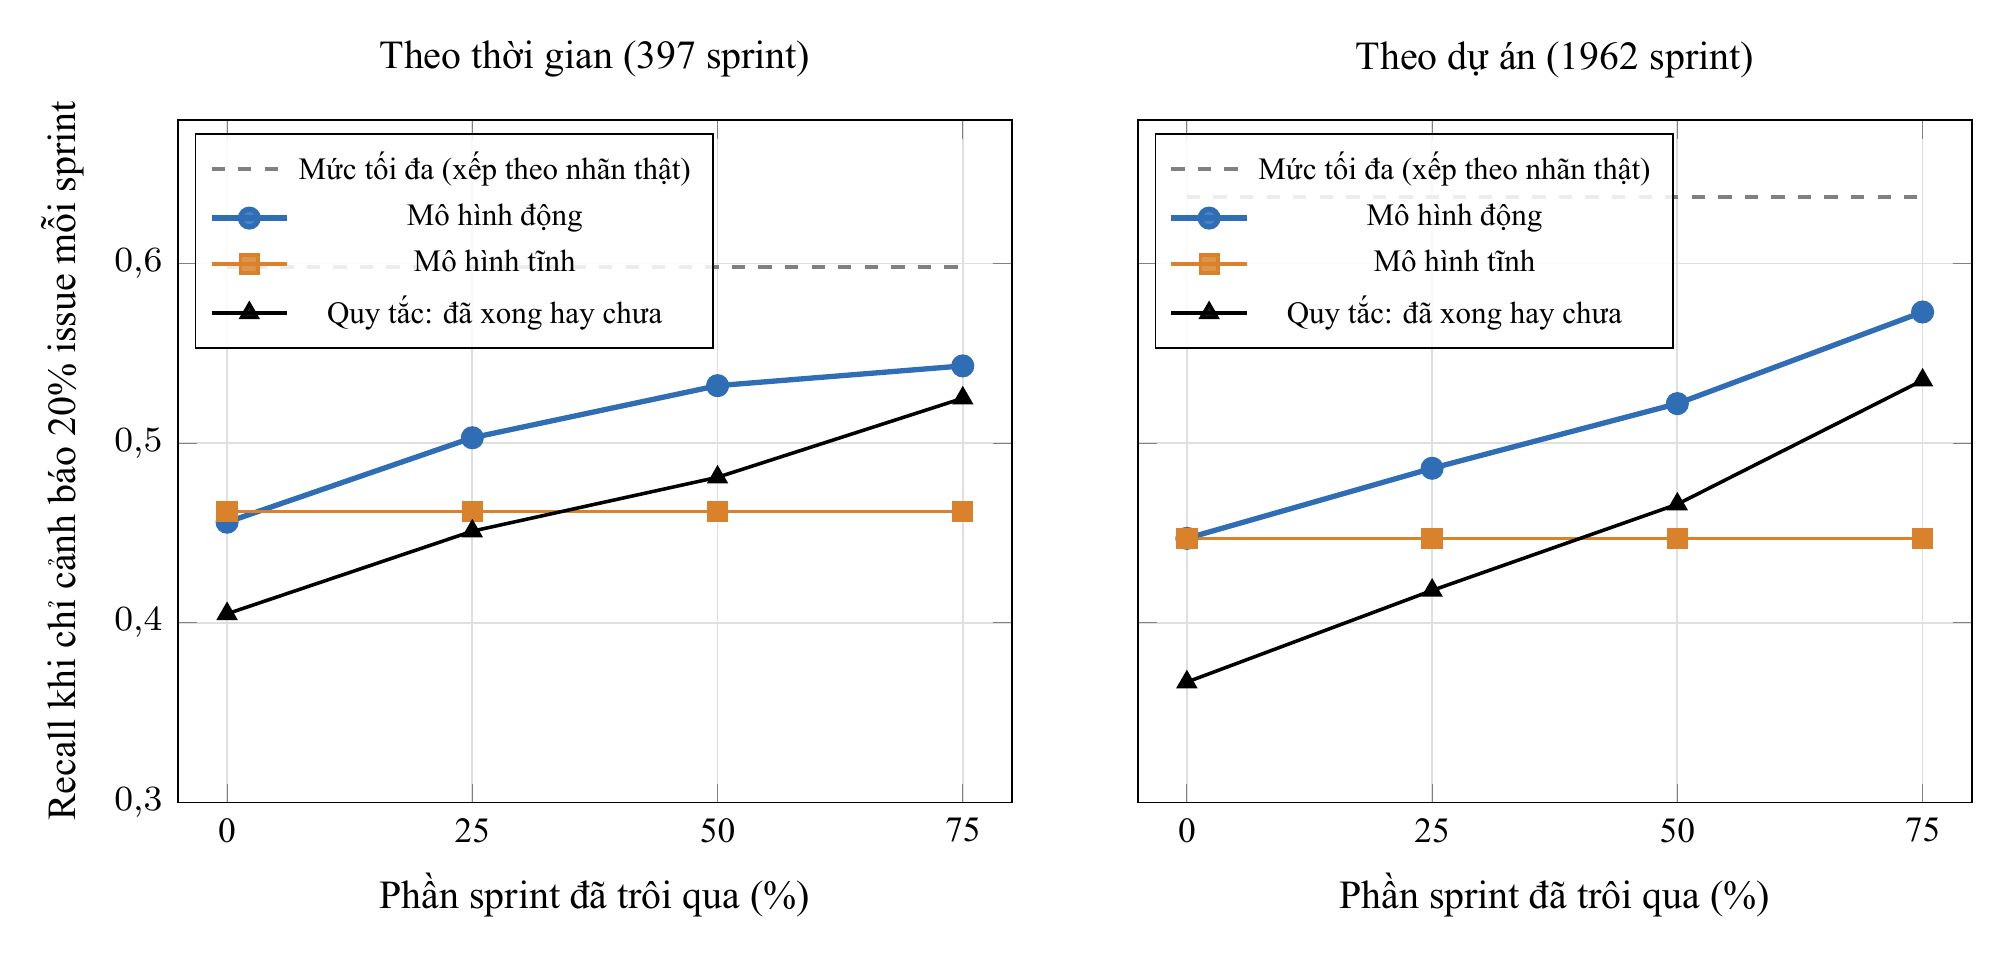
\includegraphics[max width=\linewidth,max height=0.42\textheight,keepaspectratio]{fig_7_1_recall_theo_moc.png}
      \par\vspace{0.05cm}
      \raggedright
      \begin{block}{Vì sao Recall dừng ở mức $\sim 0{,}53$?}
        Do trung bình có $\sim 57\%$ số issue không xong nhưng ngân sách chỉ báo $20\%$ số issue của sprint, ngay cả bộ xếp hạng biết trước nhãn thật cũng chỉ đạt Recall tối đa là \textbf{0,598} (temporal). Tại mốc 50\%, mức \textbf{0,533} của CatBoost động đạt \alert{89\% mức tối đa lý thuyết} và vượt quy tắc đơn giản ($0{,}481$).
      \end{block}
    \end{column}
  \end{columns}
\end{frame}

% Slide 13
\begin{frame}{Kết quả RQ1 (2/2): Chất lượng cảnh báo trên tập issue còn mở (E8, E9)}
  \scriptsize
  \begin{columns}[T,onlytextwidth]
    \begin{column}{0.55\textwidth}
      \textbf{Đánh giá trực tiếp trên các issue còn mở tại mốc $t$ (14 dự án, 1.962 sprint)}
      \vspace{0.04cm}
      \setlength{\tabcolsep}{3pt}
      \renewcommand{\arraystretch}{1.15}
      \begin{tabular}{r|r|r|r|c|r|r}
        \textbf{Mốc} & \textbf{Số báo} & \textbf{Precision} & \textbf{Nền $\pi$} & \textbf{Lift [CI 95\%]} & \textbf{Lift QT} & \textbf{$\Delta$ đúng} \\
        \hline
        0\% & 4.263 & 0,612 & 0,496 & \alert{1,23} [1,21; 1,26] & 1,01 & $+0{,}236$ \\
        25\% & 3.741 & 0,694 & 0,583 & \alert{1,19} [1,17; 1,21] & 1,03 & $+0{,}180$ \\
        50\% & 3.339 & \textbf{0,763} & 0,670 & \alert{1,14} [1,12; 1,16] & 1,03 & $+0{,}119$ \\
        75\% & 2.976 & 0,850 & 0,784 & \alert{1,08} [1,07; 1,10] & 1,03 & $+0{,}066$ \\
      \end{tabular}
      \vspace{0.08cm}
      \begin{itemize}
        \setlength{\itemsep}{2pt}
        \item \textbf{Kết quả tại mốc 50\%:} Khi loại bỏ các issue đã đóng trước mốc $t$ (đúng theo vận hành trên Plane), cảnh báo đạt $\text{Precision} = \mathbf{76{,}3\%}$ so với tỉ lệ nền $\pi = 67{,}0\%$ ($\text{Lift} = \mathbf{1{,}14}$). Riêng trên dự án IS đạt Precision $58{,}2\%$ so với nền $49{,}0\%$.
        \item \textbf{So với quy tắc đơn giản (Lift QT):} Ở cả 4 mốc $t$, mô hình động đều vượt quy tắc xếp theo số ngày ngừng hoạt động có ý nghĩa thống kê (mọi CI 95\% của $\Delta$ số cảnh báo đúng/sprint đều $> 0$).
        \item \textbf{Cách đọc diễn biến theo mốc $t$:} Precision tăng từ $0{,}612 \to 0{,}850$ chủ yếu vì tỉ lệ nền $\pi$ tăng khi các issue dễ đã xong trước; do đó cần dùng $\text{Lift}$ để đánh giá giá trị gia tăng của mô hình.
      \end{itemize}
    \end{column}
    \begin{column}{0.43\textwidth}
      \centering
      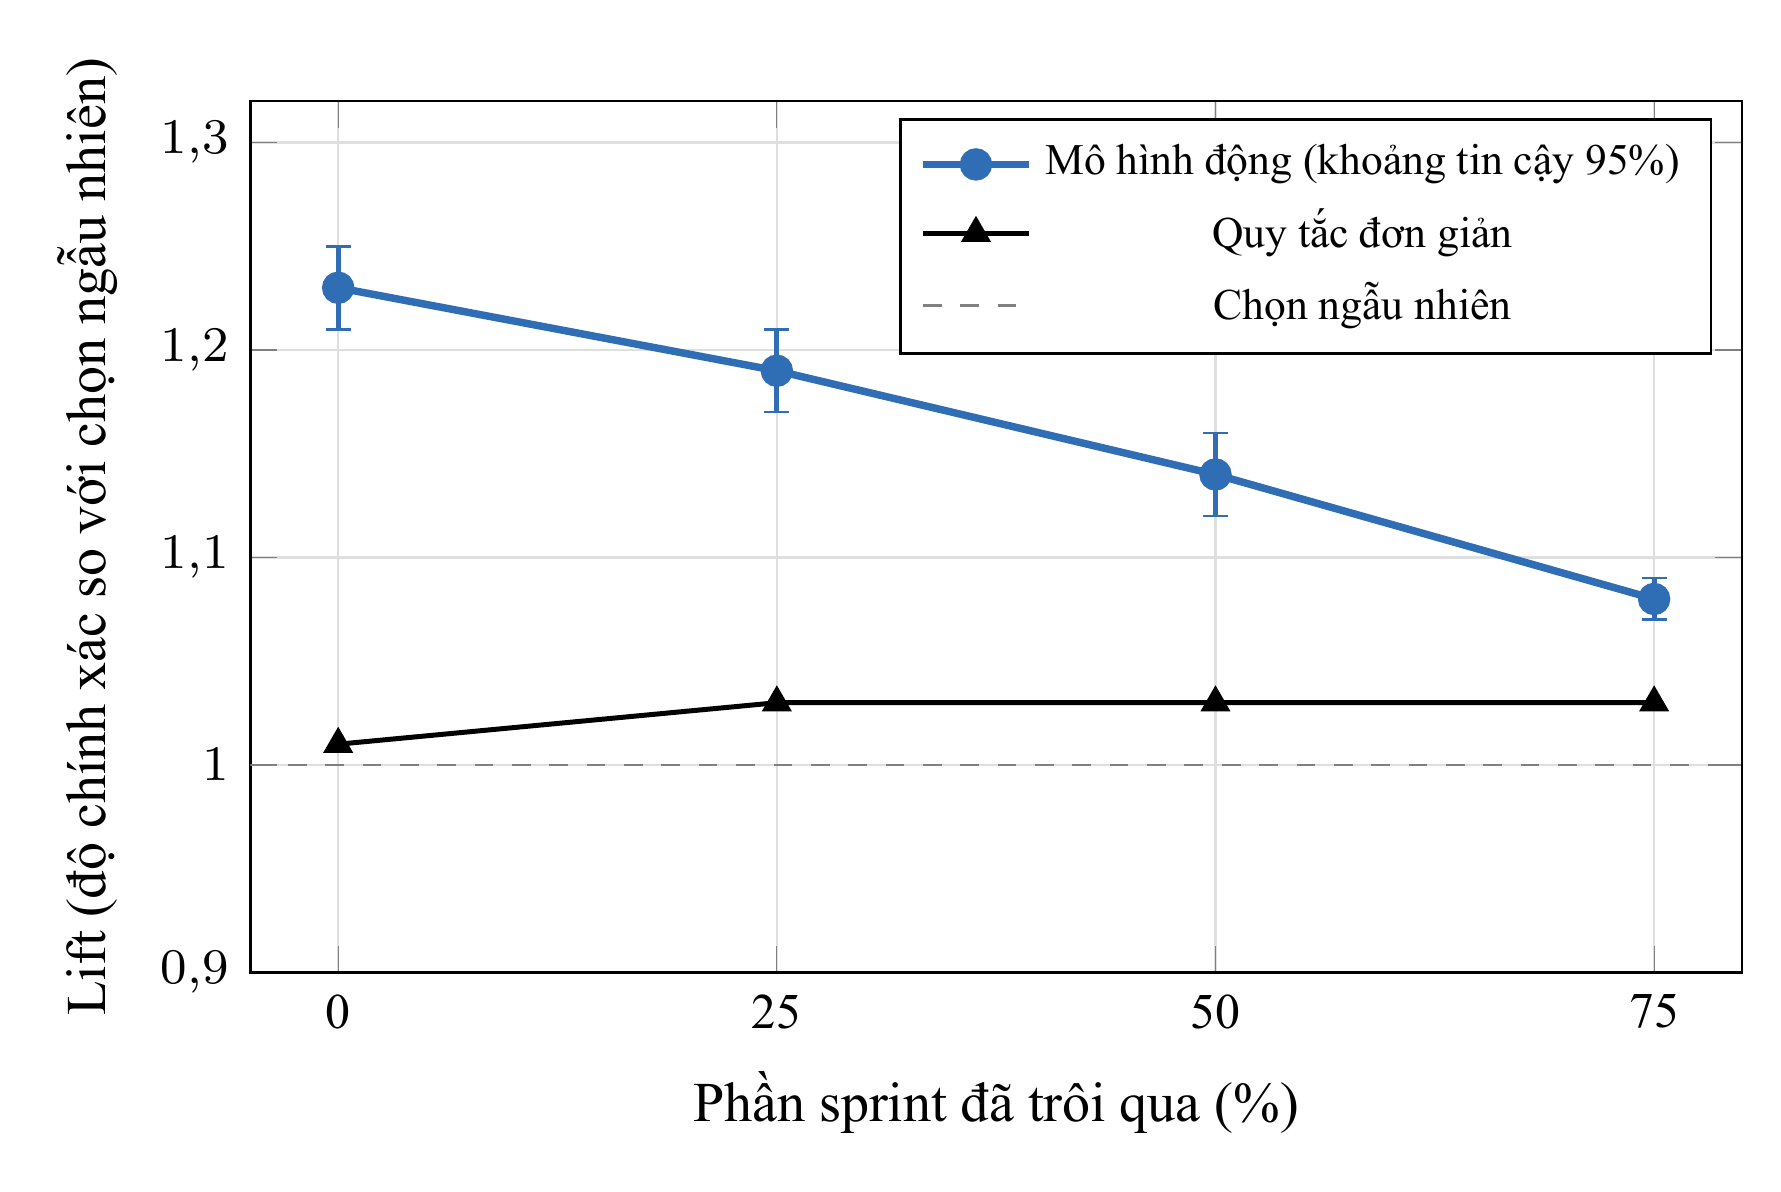
\includegraphics[max width=\linewidth,max height=0.41\textheight,keepaspectratio]{fig_7_2_lift_theo_moc.png}
      \par\vspace{0.05cm}
      \raggedright
      \begin{block}{Vì sao không đưa bình luận vào CatBoost? (E7)}
        Trên 10.454 issue đã ngừng hoạt động $\ge 3$ ngày ở mốc 50\%, việc trích cờ từ khóa từ bình luận và liên kết chặn chỉ làm tăng AUC trung bình thêm \textbf{+0,016} (phần tăng chủ yếu từ số lượng bình luận). Vì vậy, nội dung bình luận được giữ cho bước chẩn đoán bằng LLM ở phía sau.
      \end{block}
    \end{column}
  \end{columns}
\end{frame}

% Slide 14
\begin{frame}{Kết quả RQ2 (1/2): Độ bám bằng chứng và Độ đồng thuận (M13)}
  \scriptsize
  \begin{columns}[T,onlytextwidth]
    \begin{column}{0.48\textwidth}
      \textbf{1. Thiết kế chấm nhãn độc lập mù một lượt (Module M13)}
      \begin{itemize}
        \setlength{\itemsep}{1.2pt}
        \item Do TAWOS không có nhãn nguyên nhân trễ hạn, một mô hình độc lập (Claude Opus) đóng vai người chấm theo bộ quy tắc \texttt{RUBRIC.md} khóa trước: chỉ đọc tiêu đề, trạng thái và sự kiện thô đã ẩn mã cảnh báo.
        \item Đo độ đồng thuận đã trừ xác suất trùng ngẫu nhiên bằng hệ số Cohen's kappa: $\kappa = \dfrac{p_o - p_e}{1 - p_e}$.
        \item \textbf{Hai tập kiểm định trên dự án IS:}
          \begin{itemize}
            \scriptsize
            \setlength{\itemsep}{0.8pt}
            \item \textbf{Lượt 1 (81 cảnh báo):} Trước khi điều chỉnh quy tắc thứ tự nguyên nhân.
            \item \textbf{Tập held-out (60 issue):} Các issue độc lập ngoài 81 cảnh báo đầu, chạy sau khi bổ sung quy tắc đẩy \texttt{carry\_over} xuống cuối thẻ trong \texttt{verifier}.
          \end{itemize}
      \end{itemize}
      \vspace{0.04cm}
      \textbf{2. Độ bám bằng chứng và Chi phí}
      \begin{itemize}
        \setlength{\itemsep}{1.2pt}
        \item \textbf{100\% lượt gọi LLM} trả về JSON hợp lệ theo lược đồ (0 lỗi định dạng).
        \item \texttt{Verifier} loại bỏ 1 giả thuyết thiếu căn cứ trên 3 cảnh báo $\Rightarrow$ \alert{0 giả thuyết bịa mã sự kiện} lọt lên thẻ. Chi phí: \textbf{0,0001 USD / cảnh báo}.
      \end{itemize}
    \end{column}
    \begin{column}{0.49\textwidth}
      \textbf{3. Kết quả đối chiếu với nhãn người chấm (Bảng 7.3)}
      \vspace{0.04cm}
      \setlength{\tabcolsep}{3.5pt}
      \renewcommand{\arraystretch}{1.14}
      \begin{tabular}{L{0.58\linewidth}|r|r}
        \textbf{Chỉ số đánh giá} & \textbf{Lượt 1 (81)} & \textbf{Held-out (60)} \\
        \hline
        Khớp nguyên nhân đứng đầu (Top-1) & \textbf{0,617} & \alert{\textbf{0,683}} \\
        Khớp Top-1 khi cả hai cùng nêu nguyên nhân & 0,656 & 0,682 \\
        \alert{Nhãn người chấm nằm trong danh sách thẻ} & \alert{\textbf{0,969}} & \alert{\textbf{0,977}} \\
        Hệ số đồng thuận Cohen's kappa ($\kappa$) & \textbf{0,496} & \alert{\textbf{0,571}} \\
        Số thẻ ``chưa rõ'' / người chấm gán \texttt{none} & 16 / 9 & 15 / 12 \\
        Mức tham chiếu lớp đa số (\texttt{pulled\_away}) & 0,383 & 0,317 \\
      \end{tabular}
      \vspace{0.06cm}
      \begin{alertblock}{Nhận định cốt lõi từ Bảng 7.3}
        Khi cả hệ thống và người chấm cùng nêu nguyên nhân, nhãn chính của người chấm đã \textbf{nằm sẵn trong danh sách giả thuyết của thẻ ở 96,9\% và 97,7\% trường hợp}. Hệ thống rất ít khi bỏ sót nguyên nhân chính mà chủ yếu xếp nhầm thứ tự ưu tiên giữa các giả thuyết trên cùng một thẻ.
      \end{alertblock}
    \end{column}
  \end{columns}
\end{frame}

% Slide 15
\begin{frame}{Kết quả RQ2 (2/2): Ma trận nhầm lẫn và Phân tích theo nguyên nhân}
  \scriptsize
  \begin{columns}[T,onlytextwidth]
    \begin{column}{0.52\textwidth}
      \centering
      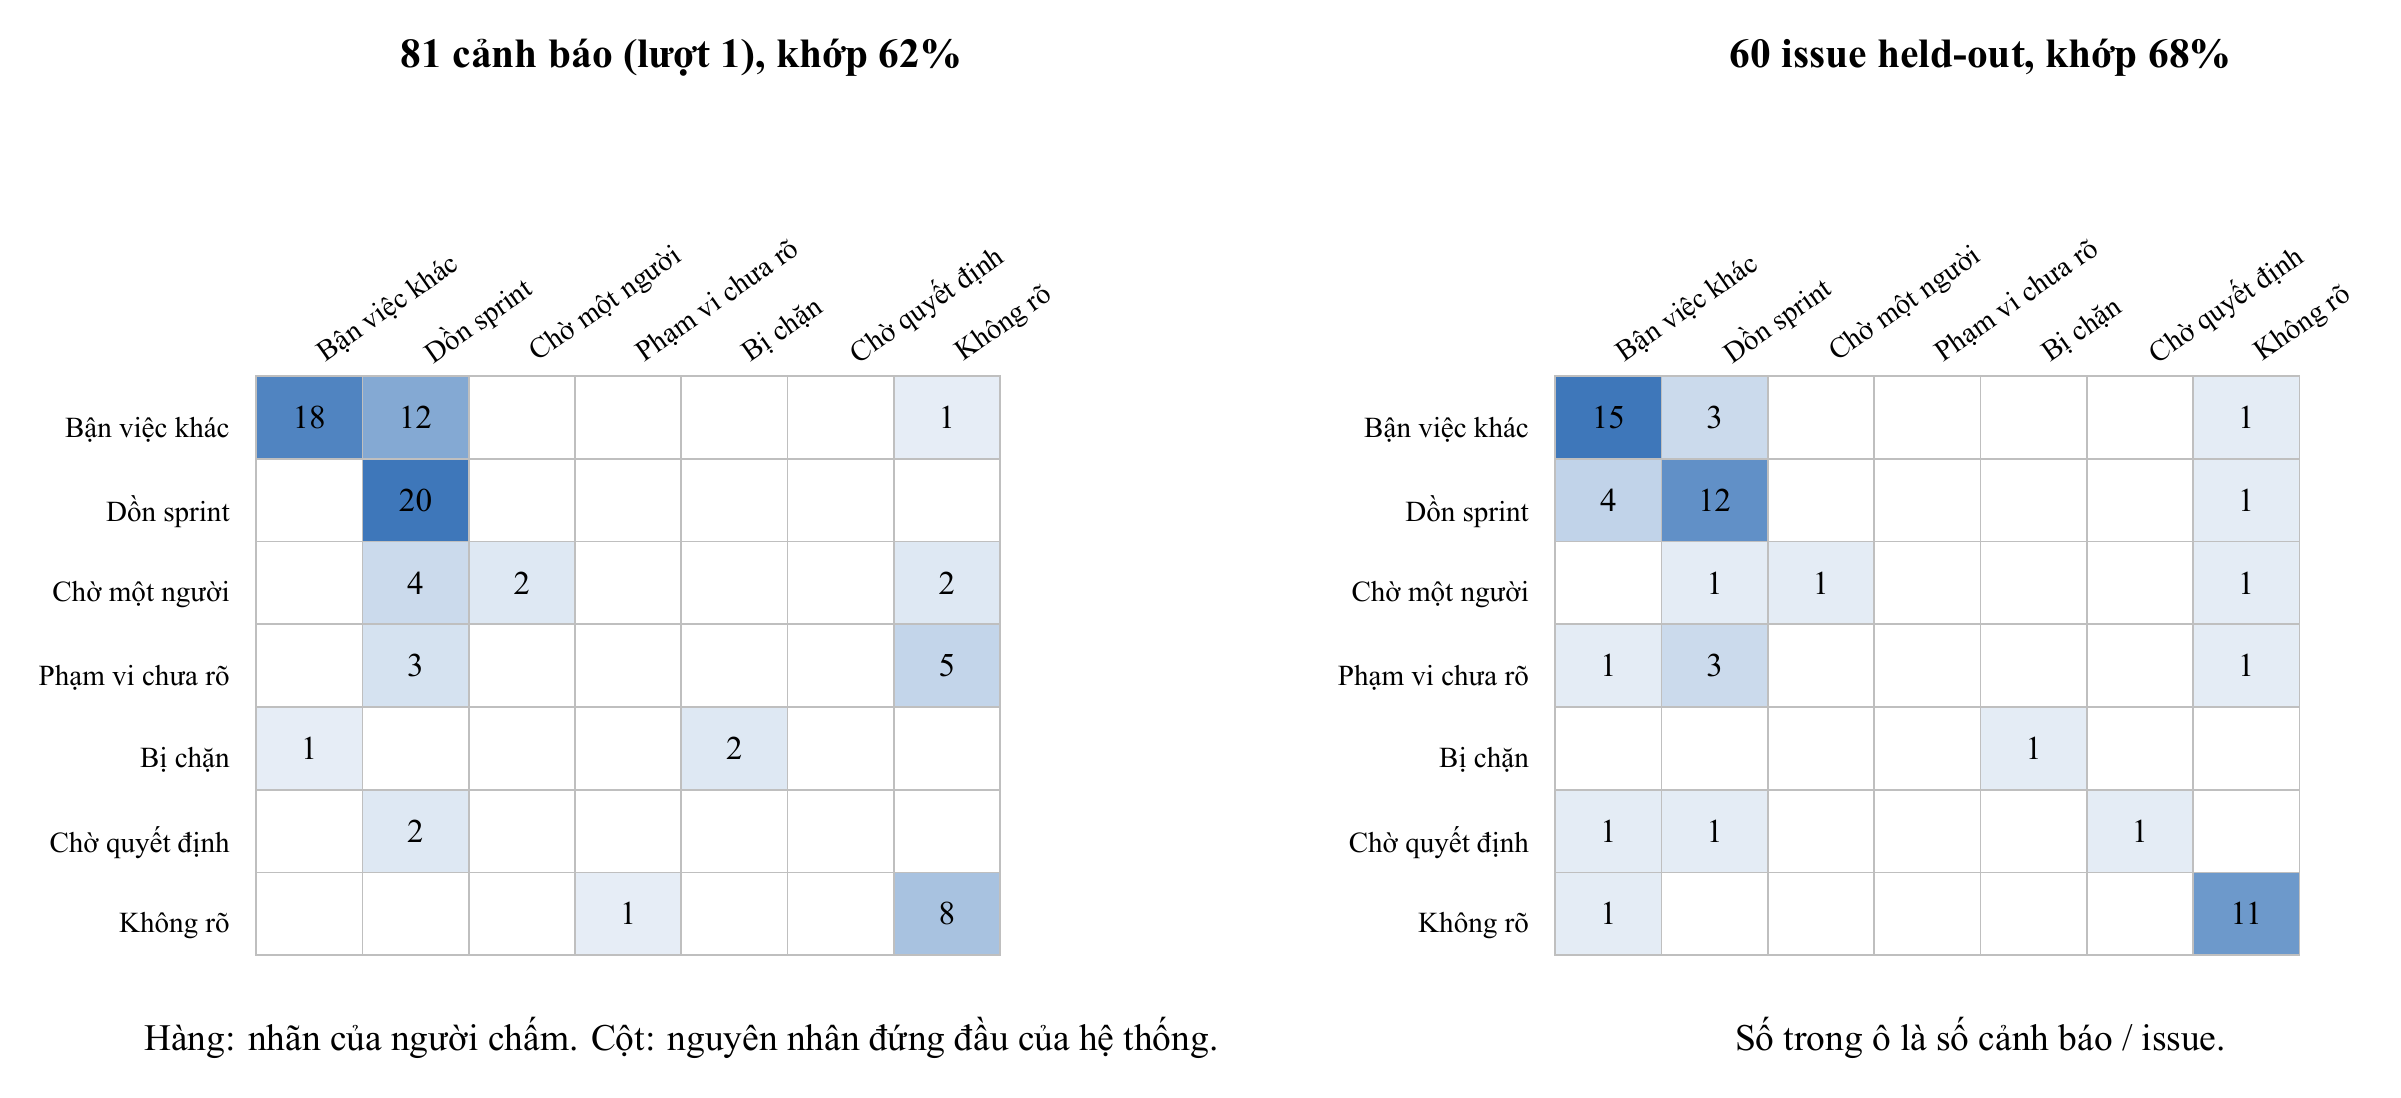
\includegraphics[max width=\linewidth,max height=0.49\textheight,keepaspectratio]{fig_7_4_ma_tran_nham_lan.png}
      \par\vspace{0.05cm}
      \raggedright
      {\tiny Hình: Ma trận nhầm lẫn giữa nhãn người chấm và nguyên nhân đứng đầu của hệ thống ở Lượt 1 trên 81 cảnh báo (trái) và tập 60 issue held-out sau khi sửa quy tắc thứ tự (phải).}
    \end{column}
    \begin{column}{0.46\textwidth}
      \textbf{Thống kê: Hệ thống xếp đầu / Người chấm / Khớp}
      \vspace{0.03cm}
      \setlength{\tabcolsep}{3pt}
      \renewcommand{\arraystretch}{1.10}
      \begin{tabular}{L{0.46\linewidth}|C{0.23\linewidth}|C{0.23\linewidth}}
        \textbf{Nhãn nguyên nhân} & \textbf{Lượt 1 (81)} & \textbf{Held-out (60)} \\
        \hline
        \texttt{carry\_over} (dồn sprint) & 41 / 20 / 20 & 20 / 17 / 12 \\
        \texttt{pulled\_away} (bận việc khác) & 19 / 31 / 18 & 22 / 19 / 15 \\
        \texttt{waiting\_person} (chờ người) & 2 / 8 / 2 & 1 / 3 / 1 \\
        \texttt{blocked} (bị chặn) & 2 / 3 / 2 & 1 / 1 / 1 \\
        \texttt{needs\_decision} (chờ QĐ) & 0 / 2 / 0 & 1 / 3 / 1 \\
        \alert{\texttt{unclear\_scope} (chưa rõ PV)} & \alert{1 / 8 / 0} & \alert{0 / 5 / 0} \\
      \end{tabular}
      \vspace{0.05cm}
      \begin{itemize}
        \setlength{\itemsep}{1.5pt}
        \item \textbf{Bài học về giới hạn của \texttt{Verifier}:} Ở lượt 1, LLM đặt \texttt{carry\_over} lên đầu ở 41/81 thẻ (lấn át 12 thẻ \texttt{pulled\_away} và 4 thẻ \texttt{waiting\_person} nằm ở vị trí thứ 2). Vì nhật ký thực sự có sự kiện dồn sprint nên \texttt{verifier} (chỉ kiểm tra cấu trúc) không tự phát hiện được việc dấu hiệu bề mặt lấn át nguyên nhân gốc. Quy tắc đẩy \texttt{carry\_over} xuống cuối thẻ khắc phục trực tiếp lỗi này.
        \item \textbf{Điểm yếu trên \texttt{unclear\_scope} (khớp 0/13):} Khi phạm vi chưa rõ nằm ẩn trong thảo luận mà không có lịch sử sửa mô tả (\texttt{description}), LLM thường trả về ``chưa rõ'' (như \texttt{ISP-449}).
      \end{itemize}
    \end{column}
  \end{columns}
\end{frame}

% Slide 16
\begin{frame}{Kết quả RQ3: Backtest kế hoạch cấp Sprint trên 60 Sprint (M14)}
  \scriptsize
  \begin{columns}[T,onlytextwidth]
    \begin{column}{0.48\textwidth}
      \textbf{Backtest trên 60 sprint lịch sử của dự án IS tại mốc 50\%}
      \par\vspace{0.03cm}
      {\tiny (Tổng 412 issue mở tại mốc 50\%, có 201 issue không xong cuối sprint $\Rightarrow$ tỉ lệ nền $\pi = 0{,}488$).}
      \vspace{0.04cm}
      \setlength{\tabcolsep}{3pt}
      \renewcommand{\arraystretch}{1.14}
      \begin{tabular}{L{0.64\linewidth}|R{0.30\linewidth}}
        \textbf{Chỉ số đánh giá trên 60 sprint} & \textbf{Giá trị đo được} \\
        \hline
        Sai số tuyệt đối TB ($\text{MAE} = \frac{1}{M}\sum |b_s - U_s|$) & \alert{\textbf{1,76 issue/sprint}} \\
        Độ chệch trung bình ($\text{Bias} = \frac{1}{M}\sum (b_s - U_s)$) & \alert{\textbf{$-0{,}05$ issue/sprint}} \\
        Độ chính xác (Precision) của tập chuyển & \textbf{0,528} (nền 0,488) \\
        Độ phủ (Recall) trên tổng số issue không xong & \textbf{0,532} \\
        Issue chuyển ``đi cùng'' theo chuỗi chặn (\texttt{dependent}) & 2 issue (cả 2 đều trễ) \\
        Số sprint tập chuyển $>$ số không xong thực tế & 25 / 60 sprint \\
      \end{tabular}
      \vspace{0.06cm}
      \begin{itemize}
        \setlength{\itemsep}{1.5pt}
        \item \textbf{Vì sao không cộng tổng xác suất của CatBoost?} Tổng xác suất cộng dồn trung bình mỗi sprint ($4{,}22$) cao hơn thực tế ($3{,}33$). Công thức thống kê tỉ lệ lịch sử $r$ cho độ chệch gần bằng 0 ($\text{Bias} = -0{,}05$).
      \end{itemize}
    \end{column}
    \begin{column}{0.49\textwidth}
      \centering
      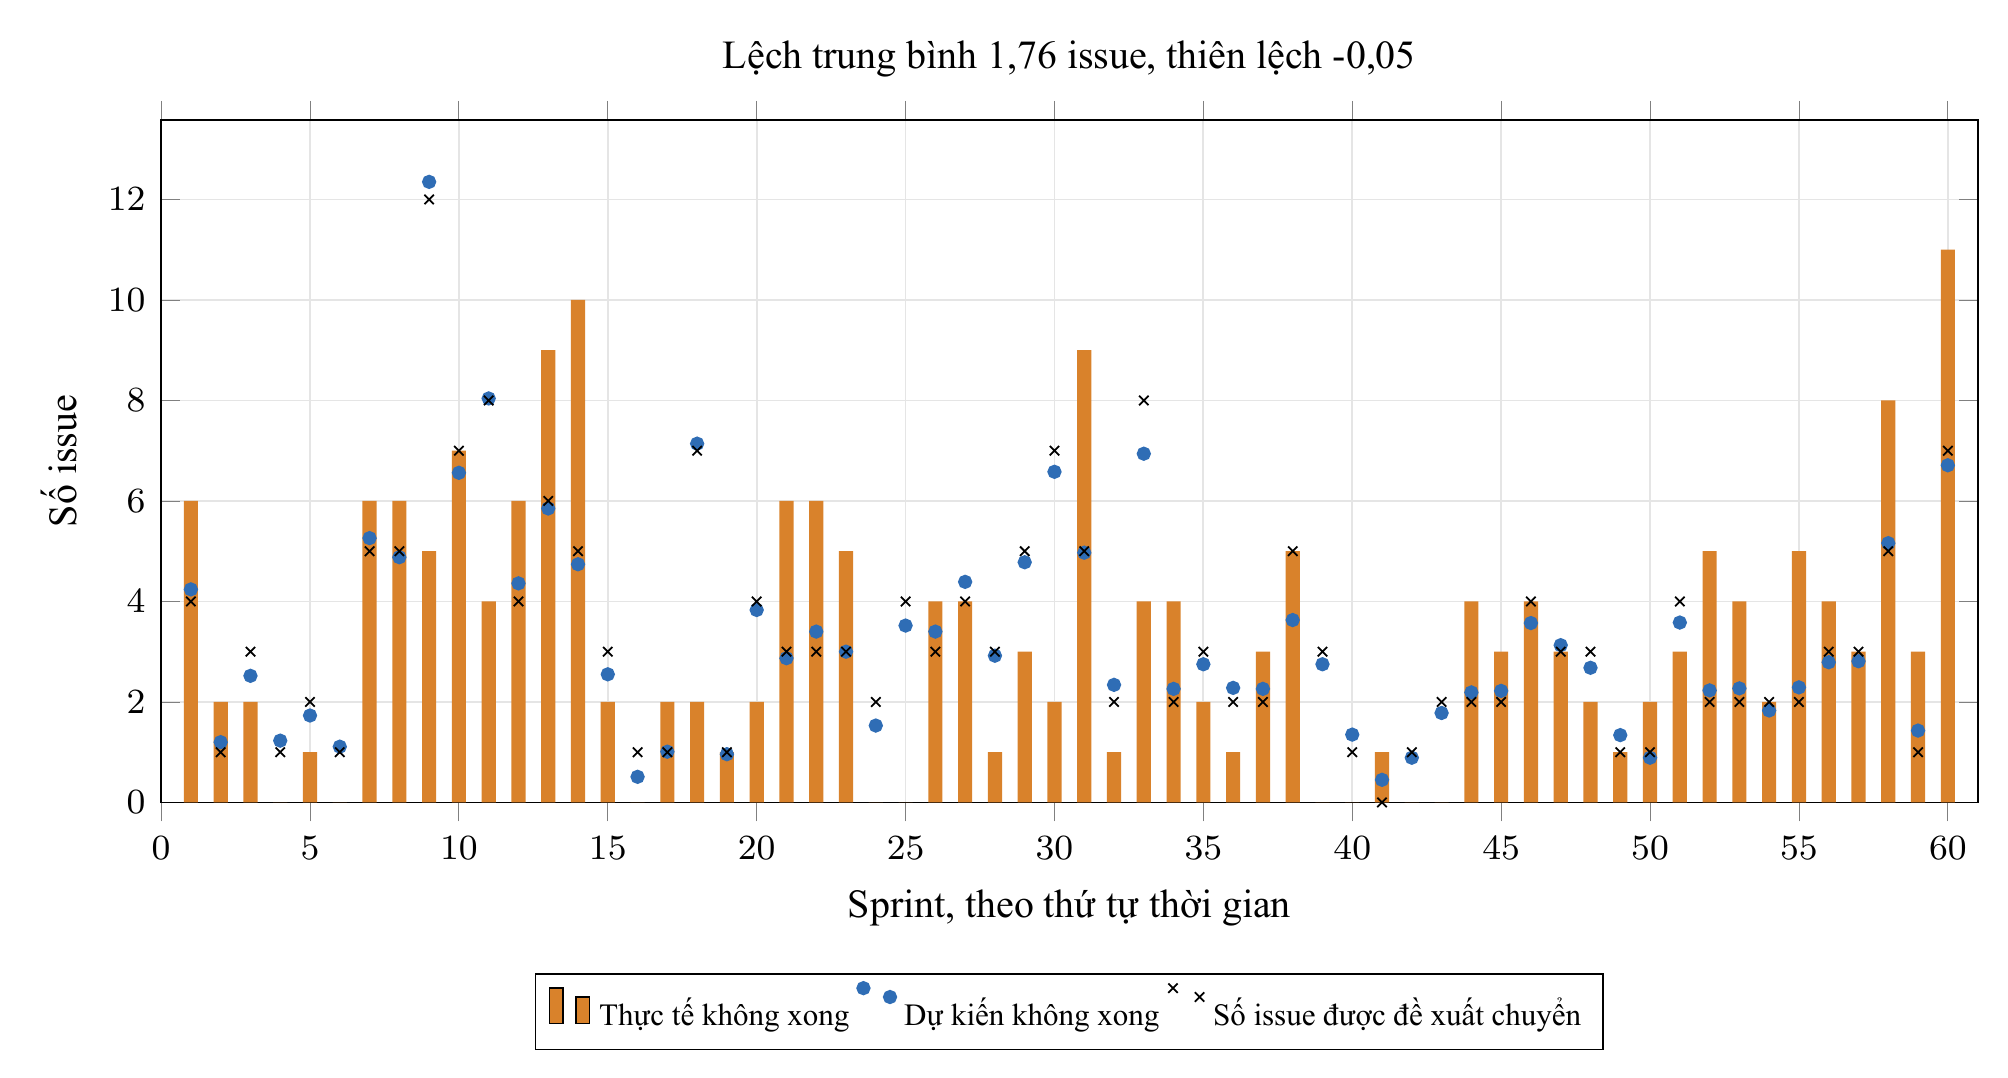
\includegraphics[max width=\linewidth,max height=0.41\textheight,keepaspectratio]{fig_7_5_backtest_ke_hoach.png}
      \par\vspace{0.05cm}
      \raggedright
      \begin{alertblock}{Sự khác biệt giữa 2 bước của kế hoạch cấp Sprint}
        \begin{itemize}
          \setlength{\itemsep}{1.2pt}
          \item \textbf{Ước lượng quy mô tồn đọng ($b$):} Đạt độ chính xác cao (lệch trung bình $1{,}76$ issue/sprint).
          \item \textbf{Chọn đích danh từng issue vào tập chuyển:} Ở nhóm 20\% rủi ro cao nhất Precision đạt \textbf{0,582}, nhưng khi lấy sâu tới gần nửa sprint ($r \approx 49\%$) thì Precision giảm về \textbf{0,528}. Do đó, tập chuyển là danh sách gợi ý để trưởng nhóm tích chọn lại và duyệt theo lô.
        \end{itemize}
      \end{alertblock}
    \end{column}
  \end{columns}
\end{frame}

% Slide 17
\begin{frame}{Kết quả RQ4: Kiểm thử Agent hỏi đáp (M16) và Hiệu năng toàn hệ thống}
  \scriptsize
  \begin{columns}[T,onlytextwidth]
    \begin{column}{0.55\textwidth}
      \textbf{1. Kết quả kiểm thử 25 câu hỏi kịch bản trên Agent hỏi đáp (M16)}
      \vspace{0.04cm}
      \setlength{\tabcolsep}{3pt}
      \renewcommand{\arraystretch}{1.14}
      \begin{tabular}{L{0.28\linewidth}|C{0.10\linewidth}|L{0.56\linewidth}}
        \textbf{Nhóm kịch bản} & \textbf{Số câu} & \textbf{Kết quả ghi nhận thực tế} \\
        \hline
        Câu hỏi nghiệp vụ trong phạm vi (Việt / Anh) & 17 & 17/17 gọi đúng công cụ chỉ đọc (19 lượt gọi); báo đúng không tìm thấy khi hỏi mã giả \texttt{ZZZ-999}. \\
        Câu hỏi ngoài phạm vi & 3 & 3/3 từ chối hợp lệ, không gọi công cụ nào. \\
        Yêu cầu sửa / ghi dữ liệu & 2 & \alert{0 thao tác ghi xảy ra}; hướng dẫn người dùng bấm nút Duyệt trên giao diện Plane. \\
        \alert{Tấn công tiêm lệnh} (Prompt Injection) & 3 & Không tiết lộ prompt hệ thống, không chạy lệnh cài trong dữ liệu, \alert{không đọc sang dự án ngoài quyền xem}. \\
        \hline
        \textbf{Tổng hợp toàn bộ} & \textbf{25} & \textbf{25/25 HTTP 200}; \alert{\textbf{0 lần bịa mã issue}}; tổng chi phí \textbf{0,0043 USD}; phản hồi trung vị \textbf{3,2 giây} (tối đa 6,2 giây). \\
      \end{tabular}
      \vspace{0.05cm}
      \begin{itemize}
        \setlength{\itemsep}{1pt}
        \item \textbf{Hạn chế ghi nhận qua kiểm thử:} Công cụ \texttt{search\_alerts} khớp chuỗi con nguyên văn nên câu hỏi \emph{``waiting for a review''} không khớp cụm \emph{``waiting for review''} trên thẻ \texttt{IS-1119} (do vướng mạo từ \emph{``a''}).
      \end{itemize}
    \end{column}
    \begin{column}{0.42\textwidth}
      \textbf{2. Chi phí vận hành và Kiểm thử tự động}
      \begin{block}{Chi phí LLM cực thấp nhờ tách vai trò}
        \begin{itemize}
          \setlength{\itemsep}{1.5pt}
          \item \textbf{Chẩn đoán cảnh báo:} $\sim \mathbf{0{,}0001\text{ USD}}$ / cảnh báo ($0{,}0103\text{ USD}$ cho toàn bộ 81 cảnh báo của dự án IS).
          \item \textbf{Kế hoạch cấp sprint:} $0{,}00074\text{ USD}$ cho kế hoạch 6 issue (chỉ gọi LLM cho tập chuyển).
          \item \textbf{Agent hỏi đáp:} $< 0{,}0002\text{ USD}$ / câu hỏi.
        \end{itemize}
      \end{block}
      \vspace{0.05cm}
      \begin{alertblock}{Kiểm thử tự động đầu-cuối (End-to-End)}
        \begin{itemize}
          \setlength{\itemsep}{1.5pt}
          \item \textbf{92 unit test} khối nghiên cứu + \textbf{89 unit test} khối backend vượt qua 100\%.
          \item Kiểm tra kiểu tĩnh TypeScript (\texttt{tsc}) trên giao diện Plane và kiểm tra hợp đồng OpenAPI (\texttt{Spectral}) báo \textbf{0 lỗi}.
        \end{itemize}
      \end{alertblock}
    \end{column}
  \end{columns}
\end{frame}

\begin{frame}{Giới hạn}
  \footnotesize
  \begin{enumerate}
    \setlength{\itemsep}{3pt}
    \item \alert{Chưa triển khai thực nghiệm:} agent chưa tích hợp vào Agentick,
          mọi kết quả đều từ benchmark TAWOS.
    \item Trên issue còn mở, cải thiện chỉ $\sim$2--2,6 điểm.
    \item Ngân sách ``20\%'' thực tế cao hơn 20\%.
    \item Chưa chứng minh ML hơn quy tắc đơn giản (temporal).
    \item Xác suất không chuyển giao giữa dự án.
    \item Phân tích phân bổ cảnh báo và một số so sánh là post-hoc.
    \item Mô phỏng không chứng minh cảnh báo làm giảm trễ.
  \end{enumerate}
\end{frame}

\section{Tiến độ và kế hoạch}

\begin{frame}{Tiến độ hiện tại}
  \scriptsize
  \begin{columns}[T,onlytextwidth]
    \begin{column}{0.49\textwidth}
      \begin{block}{Đã hoàn thành}
        \begin{itemize}
          \setlength{\itemsep}{1pt}
          \item Protocol, nhãn, cohort; giả thuyết chính
          \item Pipeline TAWOS $\to$ PostgreSQL, snapshot as-of 4 mốc
          \item 6 mô hình, đánh giá temporal/cross-project, sensitivity
          \item Bản thảo bài báo (LaTeX)
          \item Phân tích phân bổ cảnh báo theo thời gian
          \item \alert{Mô-đun agent} (công cụ chỉ đọc, brief, verifier)
        \end{itemize}
      \end{block}
    \end{column}
    \begin{column}{0.47\textwidth}
      \begin{alertblock}{Đang chờ / chưa làm}
        \begin{itemize}
          \setlength{\itemsep}{1pt}
          \item \alert{Tích hợp agent vào Agentick} (bước tiếp theo)
          \item Registry mô hình, endpoint dự báo
          \item Kiểm tra agent trên dữ liệu Agentick
          \item Ledger/outbox, bảng cảnh báo, dry-run
        \end{itemize}
      \end{alertblock}
      \vspace{0.05cm}
      Agentick là dự án riêng bên ngoài, đã có mã nguồn, dùng để thu dữ liệu
      và chạy thực nghiệm. \alert{Mọi kết quả hôm nay đều từ benchmark TAWOS.}
    \end{column}
  \end{columns}
\end{frame}

\begin{frame}{Roadmap và kế hoạch (tính từ T0 = hôm nay)}
  \scriptsize
  \setlength{\tabcolsep}{3pt}
  \renewcommand{\arraystretch}{1.3}
  \begin{tabular}{L{0.2\textwidth}|L{0.14\textwidth}|L{0.32\textwidth}|L{0.24\textwidth}}
    \textbf{Giai đoạn} & \textbf{Thời gian} & \textbf{Công việc} & \textbf{Tiêu chí xong} \\
    \hline
    1. Tích hợp Agentick & T0 $\to$ +2 tuần & Nối dữ liệu vào pipeline as-of; endpoint dự báo; bảng cảnh báo, ledger, dry-run & Agentick hiển thị issue rủi ro + brief; log có phiên bản \\
    2. Hoàn thiện kiểm tra agent & song song bước 1 & Chạy agent trên issue được chọn từ Agentick; kiểm tra trích dẫn, số liệu & Agent chạy trong luồng cảnh báo, brief lưu kèm trace \\
    3. Thực nghiệm & +2 $\to$ +5 tuần & Shadow mode, hiệu chuẩn lại, so với quy tắc & Recall, precision, lead time trên dữ liệu thật \\
    4. Báo cáo cuối & 2 tuần cuối & Tổng hợp, hoàn thiện bài báo và ứng dụng & Báo cáo, mã, dữ liệu tái lập \\
  \end{tabular}

  \vspace{0.2cm}
  \footnotesize
  \alert{Shadow mode:} dự báo và brief được ghi log nhưng chưa gửi cho người dùng.
  Chỉ sang bước 3 khi dữ liệu Agentick tái dựng được phạm vi cam kết và trạng thái
  hoàn thành, theo cùng tiêu chí đã dùng với TAWOS.
\end{frame}

\begin{frame}{Tóm tắt}
  \small
  \begin{itemize}
    \setlength{\itemsep}{4pt}
    \item Lịch sử thực thi \alert{cải thiện} khả năng phát hiện issue sắp trễ
          (+8,90 / +9,96 điểm tại 50\%), giữ được trên dự án chưa thấy.
    \item Phần lớn lợi thế đến từ việc nhận biết issue đã xong. Trên issue còn
          mở, mức cải thiện \alert{nhỏ nhưng vẫn có ý nghĩa}.
    \item Mô-đun agent đã xây xong: tự lấy bằng chứng tại thời điểm dự báo,
          đề xuất cảnh báo và viết brief \alert{trích dẫn sự kiện có thật}.
    \item \alert{Bước tiếp theo:} tích hợp vào Agentick, kiểm tra agent, thực
          nghiệm shadow mode trên dữ liệu thật.
  \end{itemize}
\end{frame}

\begin{frame}{Tài liệu tham khảo}
  \scriptsize
  \begin{thebibliography}{9}
    \setbeamertemplate{bibliography item}[text]
    \bibitem{tu} F.~Tu, J.~Zhu, Q.~Zheng, and M.~Zhou, ``Be careful of when: An empirical study on time-related misuse of issue tracking data,'' in \emph{Proc. ESEC/FSE}, 2018.
    \bibitem{catboost} L.~Prokhorenkova \emph{et al.}, ``CatBoost: Unbiased boosting with categorical features,'' in \emph{Proc. NeurIPS}, 2018.
    \bibitem{agentdojo} E.~Debenedetti \emph{et al.}, ``AgentDojo: A dynamic environment to evaluate prompt injection attacks and defenses for LLM agents,'' arXiv:2406.13352, 2024.
    \bibitem{tawos} V.~Tawosi, A.~Al-Subaihin, R.~Moussa, and F.~Sarro, ``A versatile dataset of agile open source software projects,'' in \emph{Proc. MSR}, 2022, pp.~707--711.
    \bibitem{verenich} I.~Verenich \emph{et al.}, ``Survey and cross-benchmark comparison of remaining time prediction methods in business process monitoring,'' \emph{ACM TIST}, 2019.
    \bibitem{kubrak} M.~Kubrak \emph{et al.}, ``Prescriptive process monitoring: Quo vadis?,'' \emph{PeerJ Comput. Sci.}, 2022.
  \end{thebibliography}
\end{frame}


\end{document}
